\chapter{Entropy}
\label{ch:Chapter2}
    \begin{tcolorbox}
        \paragraph{A digression:} In Problem 1.4, we came across the concept of an integrating factor. Recall that an inexact differential $\dbar z$ can be turned into an exact differential by multiplying with an integrating factor $n(x,y)$. 
        \begin{equation}
            \dbar z \longmapsto dz = n(x,y)\dbar z
        \end{equation}
    \end{tcolorbox}
    
    Now a question is that whether such an integrating factor can be written for $\dbar Q$. To answer this question, let us start from the differential of heat for an ideal gas. Here, we have two equations we can look at: Ideal gas law and the internal energy for an ideal gas.
    \begin{equation}
        PV=nR\theta \hspace{1cm} U=\frac{3}{2}nR\theta
    \end{equation}
    Using the subscript "rev" for a reversible process, we can write 
    \begin{equation}
        \dbar Q_\text{rev} = dU + PdV = \frac{3}{2}nRd\theta + \frac{nR\theta}{V}dV
        \label{eq:exactheat}
    \end{equation}  
    The second term in (\ref{eq:exactheat}) could be easily integrated had the $\theta$ term not been there. Then, let us divide the equation by $\theta$ to get
    \begin{equation}
        \frac{\dbar Q}{\theta} = \frac{3}{2}nR\frac{d\theta}{\theta} + \frac{nR}{V}dV
    \end{equation}
    Integrating this equation between an initial state $(i)$ and a final state $(f)$ of the gas, we see that LHS is now an exact differential. 
    \begin{equation}
        \int_i^f\frac{\dbar Q}{\theta} = \frac{3}{2}nR\ln\lrp{\frac{\theta_f}{\theta_i}}+nR\ln\lrp{\frac{V_f}{V_i}}
        \label{eq:exactidealheat}
    \end{equation}
    Thus, while $\dbar Q$ was an inexact differential, $\frac{\dbar Q}{\theta}$ is an exact one. Then, we can say that $1/\theta$ is an integrating factor. Let us now define a new function $S$ whose differential $dS$ is the new exact heat differential.
    \begin{equation}
        dS = \frac{\dbar Q}{\theta} \Rightarrow \int_i^f\frac{\dbar Q}{\theta} = \int_i^fdS = S_f-S_i
        \label{eq:entropy}
    \end{equation}
\newpage
    This new function is called the $\textbf{entropy}$ of the system. Combining $(\ref{eq:exactidealheat})$ and $(\ref{eq:entropy})$ we get the entropy of an ideal gas system.
    \begin{equation}
        \Delta S = \frac{3}{2}nR\ln\lrp{\frac{\theta_f}{\theta_i}}+nR\ln\lrp{\frac{V_f}{V_i}}
        \label{eq:entropydefn}
    \end{equation}
    Although we have obtained this integrating factor and defined the entropy using the ideal gas law, this expression is valid for all types of systems. Proof of this fact will not be given in this course. \\
    \\
    Consider two gases initially in two different states $(P_1,V_1,\theta_1)$ and $(P_2,V_2,\theta_2)$ separated by an adiabatic wall. When the wall is removed and enough time passes, the two gases will mix and go into a new equilibrium state $(P,V,\theta)$. This is a \textbf{spontaneous process}: A process that occurs naturally, without any outside influence. As expected, the gases will not suddenly separate and go back to their initial, non-equilibrium states. Spontaneous processes occur in a way that the entropy of the system increase. This is expressed in the Second Law of Thermodynamics.
    \begin{law*}{The Second Law of Thermodynamics}
        The sum of the entropies of the initially isolated systems is less than or equal to the total entropy of the final combination. Equaility occurs just when the two original have all their respective intensive variables equal; then the final system also has the same values.
    \end{law*}
    A corollary of the Second Law is given below.
    \begin{lawcorollary*}{Corollary 1}
        Heat spontaneously flows from a hot to a cold body.
    \end{lawcorollary*}
    The second law has many consequences and is one of the must fundamental aspects of our universe. Let us look at some of them.
    \section{The Carnot Cycle}
    \label{sec:2.1Carnotcylce}
        Imagine a spontaneous heat flow from a hot body to a cold body. If one of these bodies is much larger than the other, then the temperature of that body will not change in equal amounts to the cold one. 
        \paragraph{Reservoir / Heat Bath:} A large body whose temperature does not change upon addition of a finite temperature.
\newpage
        This flow of heat from a hot body to a cold body can be used to produce work. This work is substanially increased if the two bodies undergoing heat exchange are both reservoirs and that they do not reach an equilibrium state easily. As demonstrated in Figure (\ref{fig:engine}) this occurs as:
        \begin{itemize}
            \item $Q_H$ leaves the hot reservoir.
            \item Some system converts some of the heat into work.
            \item $Q_C$ flows from the system into the cold reservoir.
        \end{itemize}
        \begin{figure}[H]
            \centering
            \resizebox{0.6\textwidth}{!}{
            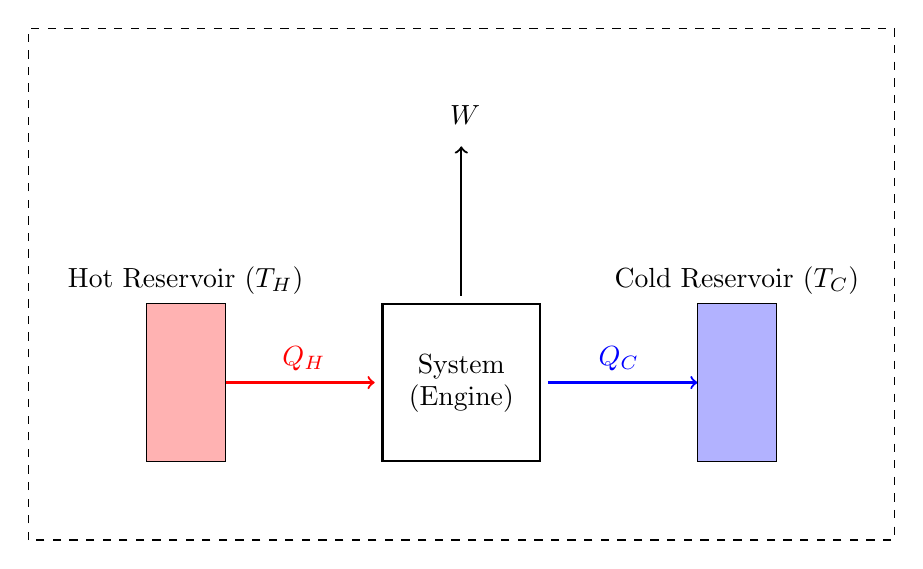
\begin{tikzpicture}
                % Hot Reservoir
                \fill[red!30] (-4, 1) rectangle (-3, -1);
                \node at (-3.5, 1.3) {Hot Reservoir ($T_H$)};
                
                % Cold Reservoir
                \fill[blue!30] (3, 1) rectangle (4, -1);
                \node at (3.5, 1.3) {Cold Reservoir ($T_C$)};
                
                % Working Substance (inside a box)
                \draw[thick] (-1, -1) rectangle (1, 1);
                \node at (0, 0.2) {System};
                \node at (0, -0.2) {(Engine)};
                %bi dk bekle olmuştu mq olum buna direkt system yazak bi de rezrvuarların contourlarını düz çizgi yapsana dashed olmasın yaptım bi de carnot cycle'ı sil genel bi engine olsun bu
                % Heat flow from Hot Reservoir to Working Substance
                \draw[->, thick, red] (-3, 0) -- (-1.1, 0);
                \node[red] at (-2, 0.3) {$Q_H$};
                
                % Heat flow from Working Substance to Cold Reservoir
                \draw[->, thick, blue] (1.1, 0) -- (3, 0);
                \node[blue] at (2, 0.3) {$Q_C$};
                
                % Work done by the engine
                \draw[->, thick, black] (0, 1.1) -- (0, 3);
                \node[black] at (0.05, 3.4) {$W$};
            
                % Carnot Cycle Box
                \draw[dashed] (-5.5, -2) rectangle (5.5, 4.5);
                \node at (-3.5, 3) {};
                % Hot resevoir contour
                \draw[-] (-4, -1) rectangle (-3, 1);
                \node at (-3.5, 3) {};
                % Hot resevoir contour
                \draw[-] (3, -1) rectangle (4, 1);
                \node at (-3.5, 3) {};
            \end{tikzpicture}
            }
            \caption{Diagram of a basic heat engine.}
            \label{fig:engine}
        \end{figure}
        
        \paragraph{Heat Engine: } A system that operates between a hot and a cold reservoir, producing work. \\
        In an ideal heat engine, the work produced equals the difference between the heat transferred between the engine and the reservoirs. Thus, all of the heat difference is converted to work.
        \begin{equation}
            W = Q_H - Q_C
        \end{equation}
        The \textbf{efficiency} of such an engine is defined as
        \begin{equation}
            \eta = \frac{W}{Q_H}
        \end{equation}
        By definition, we see that the efficiency can never be $100\%$. Such a case would require $Q_C=0$. A question is then: What is the highest efficiency engine one can define? For this, an engine must operate in a cyclical manner so that it is reusable. Such an engine is called a \textbf{Carnot engine}: A cyclical engine that is made up of four reversible processes. 
        \begin{enumerate}
            \item Isothermal expansion. A heat input of $Q_1$ is applied. Since the process is isothermal, internal energy is constant. $P\propto V^{-1}$.
            \item Adiabatic expansion. $\Delta Q=0$. $P\propto V^{-\gamma}$.
            \item Isothermal compression. Heat $Q_2$ is taken out of the system. The internal energy is constant. $P\propto V^{-1}$.
            \item Adiabatic compression. $\Delta Q = 0$. $P\propto V^{-\gamma}$. 
        \end{enumerate}
        This cycle is called the \textbf{Carnot cycle}. Since this engine is reversible, it can be run backwards. 

        \begin{figure}[t]
            \centering
                \begin{tikzpicture}
                [
                % Corner style
                    corner/.style={ 
                        circle,
                        fill,   
                        inner sep=1pt},
                % Line with Arrow style
                    arrowline/.style={
                        thick,
                        postaction = decorate,
                        decoration = {markings,
                            mark = at position .6 with \arrow{latex}
                        }
                    }]
                % Draw axis with labels
                \draw [latex-latex] (0,5)  |- (8,0) 
                    node [pos=.95,below] {V}
                    node [pos=0.07,left] {P};
                 
                % Cycle corners
                \node[corner,
                    label = {left:$1$}] (1) at (1,4.5){} ;
                 
                \node[corner,
                    label = {right:$2$}] (2) at (4,3.5){} ;
                 
                \node[corner,
                    label = {right:$3$}] (3) at (5,1){} ;
                 
                \node[corner,
                    label = {below left:$4$}] (4) at (1.5,2){} ;
                 
                % Curved lines
                \draw [name path = A, arrowline,blue!70] (1) to [bend right = 15] 
                    node [pos = .4] {} (2);
                 
                \draw [name path = B, arrowline,red!70 ] (2) to [bend right = 15] 
                    node [pos = .4] {}(3);
                 
                \draw [name path = C, arrowline,blue!70] (3) to [bend left  = 15] 
                    node [pos = .4] {} (4);
                 
                \draw [name path = D, arrowline,red!70 ] (4) to [bend left  = 15] 
                    node [pos = .4] {} (1);

                % Heat input and output
                \draw[->, thick, black] (3.2, 4.47) -- (3.2, 3.67
                );
                \node[black] at (3.5, 4.4) {$Q_1$};
                \draw[->, thick, black] (3.2, 1) -- (3.2, 0.3);
                \node[black] at (2.9, 0.3) {$Q_2$};
                % Work
                \fill[blue!20,opacity=0.7] (1) to [bend right=15] (2) to [bend right=15] (3) to [bend left=15] (4) to [bend left=15] (1);
                \node[black] at (2.7,2.7) {$W$};
                \end{tikzpicture}
            \caption{P-V plot of the Carnot engine.}
            \label{fig:carnotcycle}
        \end{figure}
        $P-V$ diagram of these processes are given in Fig (\ref{fig:carnotcycle}). The area between these four curves gives the work obtained from the engine. Moreover, since the overall change in the internal energy is zero, $W=\Delta Q = Q_1-Q_2$. Therefore, the efficiency is 
        \begin{equation}
            \eta = \frac{W}{Q_1}= 1-\frac{Q_2}{Q_1} < 1.
        \end{equation}
        This shows that an engine with $100\%$ efficiency is not possible. Other than being the simplest engine, Carnot engine has one more important property.
        \begin{theorem}{Carnot Theorem}
            bThe most efficient engine is the Carnot engine.
        \end{theorem}
        Now let us prove this theorem. There are two parts to this proof: \\
        \begin{wrapfigure}{l}{0.5\textwidth}
            \centering
            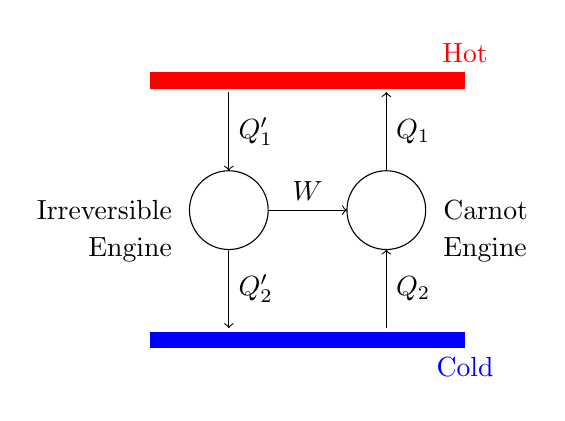
\begin{tikzpicture}
                % Draw the hot and cold reservoirs
                \draw[line width=6pt, red] (-2,1.65) -- (2,1.65) node[above] {\textcolor{red}{Hot}};
                \draw[line width=6pt, blue] (-2,-1.65) -- (2,-1.65) node[below] {\textcolor{blue}{Cold}};
            
                % Draw the circles for the Carnot engine and evaporative engine

                \draw (-1,0) circle (0.5) node[left=0.6cm] {Irreversible};
                \draw (-1,-0.5)  node[left=0.6cm] {Engine};
                \draw (1,0) circle (0.5) node[right=0.6cm] {Carnot};
                \draw (1,-0.5)  node[right=0.6cm] {Engine};                
            
                % Draw the arrows and labels
                \draw[->] (-1,1.5) -- (-1,0.5) node[midway,right] {$Q_1'$};
                \draw[<-] (1,1.5) -- (1,0.5) node[midway,right] {$Q_1$};
                \draw[->] (-1,-0.5) -- (-1,-1.5) node[midway,right] {$Q_2'$};
                \draw[<-] (1,-0.5) -- (1,-1.5) node[midway,right] {$Q_2$};
                \draw[->] (-0.5,0) -- (0.5,0) node[midway,above] {$W$};
            
                % Add labels for heat flow directions
                \node at (0,2.2) {};
                \node at (0,-2.2) {};
             \end{tikzpicture}
             \caption{An irreversible engine and a Carnot engine sharing the same reservoirs.}
             \label{fig:irrevcarnot}
        \end{wrapfigure}
        First we have to prove that no irreversible engine is more efficient than the Carnot engine, given that both engines run between the same reservoirs. As seen in Figure (\ref{fig:irrevcarnot}), the irreversible engine is used to run the Carnot engine backwards. Then,
        \begin{equation}
            \eta_I = \frac{W}{Q_1'} \hspace{0.6cm} \eta_C = \frac{W}{Q_1}.
        \end{equation}
        Note that for the efficiency of the Carnot engine, we have used $Q_1$ despite the engine running from the cold reservoir to the hot one. When calculating the efficiency, what matters is the heat corresponding to the hot reservoir, no matter the direction. Let us first assume that the efficiency of the irreversible engine is larger than the Carnot engine. 
        \begin{equation}
            \eta_I > \eta_C \Rightarrow \frac{W}{Q_1'} > \frac{W}{Q_1} \Rightarrow Q_1 > Q_1'
        \end{equation}
        If this is the case, this means that the heat flow into the reservoir $\Delta Q = Q_1-Q_1'$ is positive. This contradicts the Second Law and thus we prove by contradiction that no irreversible engine can have a larger efficiency than a Carnot engine.
        
        For the second part, we must prove that all Carnot engines have the same efficiency given that they operate with same temperatures. Again let us assume two Carnot engines with the same setup as in Figure (\ref{fig:irrevcarnot}) with $Q_1' \neq Q_1$. Since both engines are reversible, we have two cases.
        \begin{enumerate}
            \item $Q_1'>Q_1$: The forward composite engine obeys the Second Law but the backward one does not. 
            \item $Q_1'<Q_1$: The forward composite engine does not obey the Second Law. 
        \end{enumerate}
        Since both cases lead to a violation of the Second Law, two engines must have the same heat flowing from/to the hot reservoir. Therefore, both engines must have the same efficiency. This means that all Carnot engines have the same efficiency regardless of what system they are made of. Their efficiency only depends on the temperatures of the reservoirs. 
        
        Combining these two proofs, we show that the most efficient engine is indeed the Carnot engine.
        
        Now, let us determine the functional dependence of the efficiency. 
        
        \begin{equation}
            \eta = \frac{Q_1-Q_2}{Q_1} = 1-\lrp{\frac{Q_1}{Q_2}}^{-1} \Rightarrow \frac{Q_1}{Q_2} = \frac{1}{1-\eta}
        \end{equation}
        
        Since the heats depend only on the temperatures $\theta_1$ and $\theta_2$ of the reservoirs, we define a function $f(\theta_1,\theta_2) = \frac{Q_1}{Q_2}$.\\
        \begin{wrapfigure}{r}{0.4\textwidth}
            \centering
            \resizebox{0.32\textwidth}{!}{
            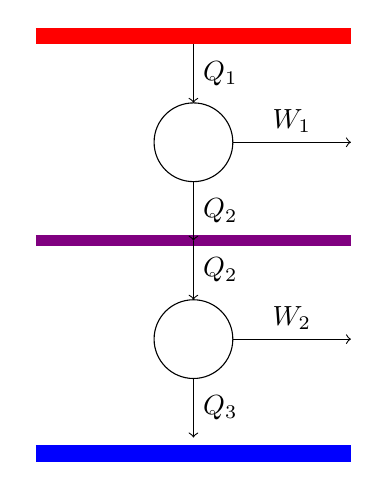
\begin{tikzpicture}
                % Draw the hot, middle, and cold reservoirs with thicker and colored lines
                \draw[line width=6pt, red] (-2,2.1) -- (2,2.1);
                \draw[line width=4pt, violet] (-2,-0.5) -- (2,-0.5);
                \draw[line width=6pt, blue] (-2,-3.2) -- (2,-3.2);
            
                % Draw the circles for the engines
                \draw (0,0.75) circle (0.5);
                \draw (0,-1.75) circle (0.5);
            
                % Draw the arrows and labels for the top engine
                \draw[->] (0,2) -- (0,1.25) node[midway,right] {$Q_1$};
                \draw[->] (0.5,0.75) -- (2,0.75) node[midway,above] {$W_1$};
                \draw[->] (0,0.25) -- (0,-0.5) node[midway,right] {$Q_2$};
            
                % Draw the arrows and labels for the bottom engine
                \draw[->] (0,-0.50) -- (0,-1.25) node[midway,right] {$Q_2$};
                \draw[->] (0.5,-1.75) -- (2,-1.75) node[midway,above] {$W_2$};
                \draw[->] (0,-2.25) -- (0,-3) node[midway,right] {$Q_3$};
            \end{tikzpicture}}              
            \caption{Two Carnot engines connected in series with three reservoirs.}
            \label{fig:twocarnots}
        \end{wrapfigure}
        \begin{equation}
            \frac{Q_1}{Q_3} = \frac{Q_1}{Q_2}\frac{Q_2}{Q_3}
        \end{equation}
        \begin{equation}
            \Rightarrow f(\theta_1,\theta_3) = f(\theta_1,\theta_2)f(\theta_2,\theta_3)
        \end{equation}
        To ensure that $\theta_2$ disappears from the equations, the functions must then take the form $f(\theta_i,\theta_j)=\phi(\theta_i)/\phi(\theta_j)$. Then,
        \begin{equation}
            f(\theta_1,\theta_3) = \frac{\phi(\theta_1)}{\phi(\theta_3)}
        \end{equation}
        so that 
        \begin{equation}
             \frac{Q_1}{Q_3} = \frac{\phi(\theta_1)}{\phi(\theta_3)}
        \end{equation}
\newpage
        This result determines a temperature scale called \textbf{Kelvin Scale}.
        \begin{equation}
            \frac{Q_1}{Q_2} = \frac{T_1}{T_2}
        \end{equation}
        Here, $T_1 \equiv \phi(\theta_1)$ is the definition of the \textbf{Kelvin temperature}. Now, if we set the lower temperature to some well known value we can determine $T_2$ with respect to this value. Let us assume an ideal gas and see how the Kelvin scale relates to the ideal gas temperature. For this, let us go through the full Carnot cycle. In the isothermal processes,
        \begin{equation}
            dU = 0 = \dbar Q - PdV \Rightarrow \dbar Q = PdV.
        \end{equation}
        Then the heat coming in is:
        \begin{equation}
            Q_1 = \int_A^B PdV = nR\theta_1\int_{V_A}^{V_B}\frac{dV}{V} = nR\theta_1\ln\lrp{\frac{V_B}{V_A}}.
        \end{equation}
        Similarly, the heat leaving the system is:
        \begin{equation}
            Q_2 = \int_C^DPdV = nR\theta_2\ln\lrp{\frac{V_D}{V_c}}.
        \end{equation}
        Let us take $Q_2$ to be positive for a while. Since $V_D<V_C$, 
        \begin{equation}
            Q_2 = nR\theta_2\lrp{\frac{V_C}{V_D}}.
        \end{equation}
        Then,
        \begin{equation}
            f(\theta_1,\theta_2) =\frac{T_1}{T_2} = \frac{Q_1}{Q_2} = \frac{nR\theta_1\ln\lrp{V_B/V_A}}{nR\theta_2\ln\lrp{V_C/V_D}} = \frac{\theta_1\ln\lrp{V_B/V_A}}{\theta_2\ln\lrp{V_C/V_D}}.
            \label{eq:kelvinfunc}
        \end{equation}
        Next, we need the relation between volumes. During the adiabatic portions, 
        \begin{equation}
            PV^\gamma = \text{const} \hspace{0.5cm} \text{or} \hspace{0.5cm} \theta V^{\gamma-1}=\text{const}.
        \end{equation}
        Since the $B$ and $C$ are connected through adiabatic processes, 
        \begin{equation}
            \theta_1V_B^{\gamma-1} = \theta_2V_C^{\gamma-1}.
            \label{eq:adiabatic1}
        \end{equation}
        Same also applies to points $D$ and $A$.
        \begin{equation}
            \theta_1V_A^{\gamma-1} = \theta_2V_D^{\gamma-1}
            \label{eq:adiabatic2}
        \end{equation}
        Dividing Equation (\ref{eq:adiabatic1}) by (\ref{eq:adiabatic2}) and taking the logarithm we get,
        \begin{equation}
            (\gamma-1)\ln\lrp{\frac{V_B}{V_A}} = (\gamma-1)\ln\lrp{\frac{V_C}{V_D}}
        \end{equation}
        Substituting this into Equation (\ref{eq:kelvinfunc}),
        \begin{equation}
            \frac{Q_1}{Q_2} = \frac{\theta_1\ln\lrp{V_B/V_A}}{\theta_2\ln\lrp{V_B/V_A}} = \frac{\theta_1}{\theta_2}.
        \end{equation}
        Now with the Kelvin scale, letting $\theta_1 = \theta$ and $\theta_2=\theta_0$
        \begin{equation}
            \frac{T}{T_0} = \frac{\theta_1}{\theta_2} = \frac{\theta}{\theta_0} \Rightarrow T = \theta\lrp{\frac{T_0}{\theta_0}}
        \end{equation}
        This shows that the ideal gas temperature is proportional to the Kelvin temperature. We can choose this constant of proportionality to be 1 and replace $\theta$ with $T$. From now on, we will use the Kelvin scale.
    \section{Definition of Entropy}
    \label{sec:2.2Definitionofentropy}
        We start this section by changing our convention: The heat that exits the system will take a negative sign. We have, therefore,
        \begin{equation}
            \frac{Q_1}{-Q_2} = \frac{T_1}{T_2} \Rightarrow \frac{Q_1}{T_1} + \frac{Q_2}{T_2} = 0
            \label{eq:heatflow}
        \end{equation}
        This is the \textbf{equation of heat flow} in a Carnot cycle. Let us now consider a general reversible closed cycle and analyse it in terms of infinitesimal Carnot cycles. 
        \begin{figure}[H]
            \centering
            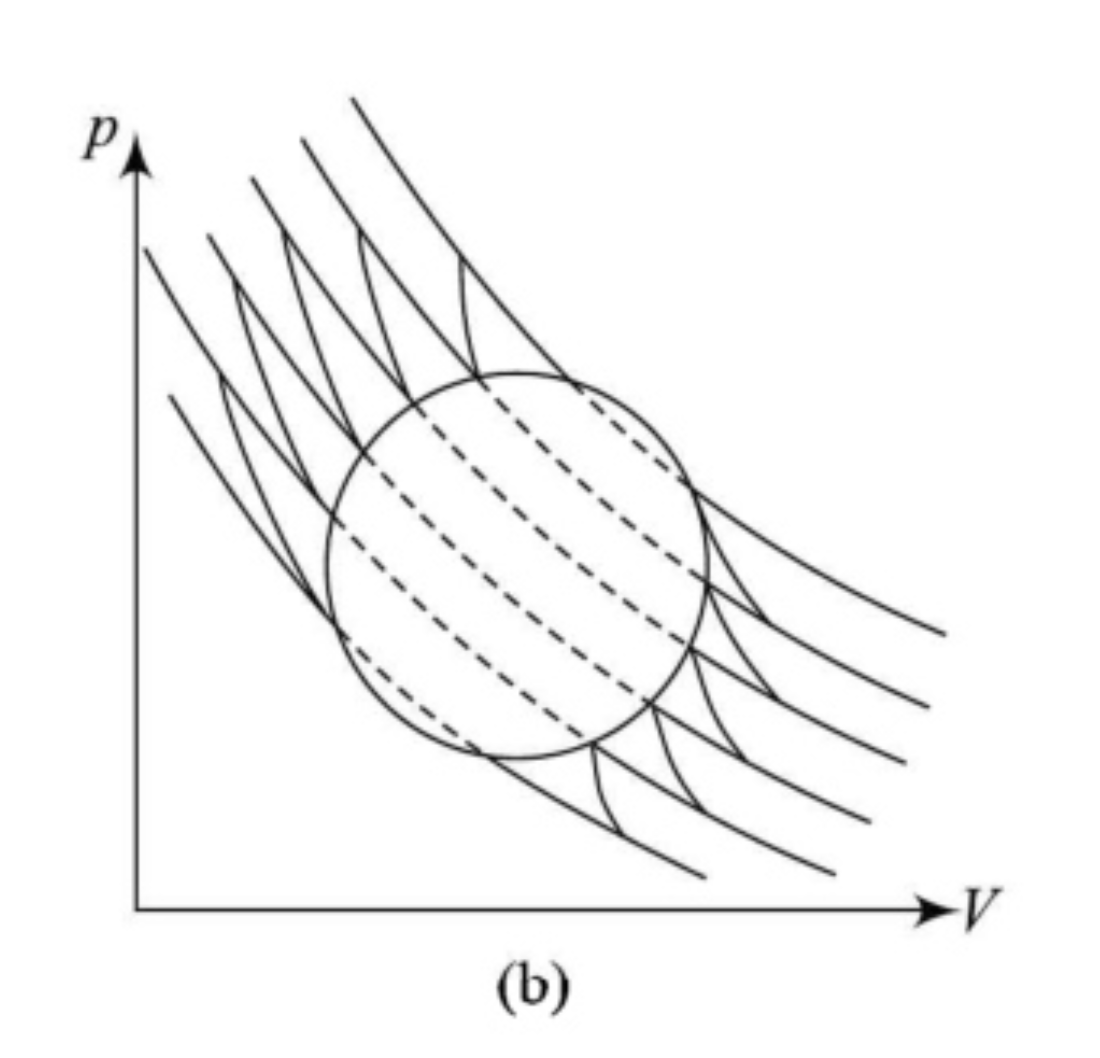
\includegraphics[width = 0.4\textwidth]{Entropy_Carnot.png}
            \caption{A general reversible closed cycle in terms of infinitesimal Carnot cycles.}
            \label{fig:generalcycle}
        \end{figure}
        In Figure (\ref{fig:generalcycle}), we have many isothermal and adiabatic stages where the work done in opposite directions cancel each other out. For an infinitesimally small Carnot engine, Equation (\ref{eq:heatflow}) becomes
        \begin{equation}
            \frac{\dbar Q_1}{T_1} + \frac{\dbar Q_2}{T_2} = 0,
        \end{equation}
        which when summed over all Carnot cycles in the continuous limit gives us
        \begin{equation}
            \sum_i\frac{\dbar Q_i}{T_i} = 0 \longmapsto \oint\frac{\dbar Q_\text{rev}}{T} = \Delta S = 0
        \end{equation}
        Therefore, the entropy of a system in a reversible closed cycle is conserved.\\
        Looking at the entropy differential, we see that $TdS = \dbar Q_\text{rev}$. Thus, we can rewrite the internal energy as
        \begin{equation}
            dU = \dbar Q_\text{rev} - dW = TdS - PdV.
        \end{equation}
        By this definition, we can relate the heat capacities to the entropy. Recall that
        \begin{equation}
            C_V = \lrp{\frac{\dbar Q_\text{rev}}{dT}}_V,
        \end{equation}
        then
        \begin{equation}
            C_V = T\lrp{\periv{S}{T}}_V.
        \end{equation}
        Similarly,
        \begin{equation}
            C_P = T\lrp{\periv{S}{T}}_P.
        \end{equation}
        Consider the entropy change in a reversible process at constant pressure.
        \begin{equation}
            \Delta S = \int_i^f\frac{\dbar Q_\text{rev}}{T} = \int_{T_i}^{T_f}C_P(T)\frac{dT}{T}
        \end{equation}
        If the system has a nearly constant $C_P$ over the temperature range of the integral then we get
        \begin{equation}
            \Delta S = C_P\ln\lrp{\frac{T_f}{T_i}}.
        \end{equation}
        A good phenomenon to derive the results that we can use to measure the entropy is the phase transitions. During phase transitions, the system takes in heat but the temperature doesn't change. For a phase transition at constant pressure, we can use the enthalpy function defined in (\ref{sec:1.4thermodynamicfunctions}).
        \begin{equation}
            \Delta H = \Delta(U+PV) = \Delta U + P\Delta V
        \end{equation}
        \begin{equation}
            \Delta U = \Delta Q - P\Delta V \Rightarrow \Delta Q = \Delta U +P\Delta V = \Delta H
        \end{equation}
        \begin{equation}
            \Delta S = \frac{\Delta Q_p}{T_p}=\frac{\Delta H}{T_p}
        \end{equation}
        Therefore, all the heat input goes to increase the enthalpy of the system. We can see a complete phase transition (for example of water) in Figure (\ref{fig:phasetransition})
        \begin{figure}[H]
            \centering
            \begin{tikzpicture}
                  \def\ymin{-0.8}
                  \def\ymax{3}
                  \def\xmin{-0.2}
                  \def\xmax{7}
                  \def\t{0.3}    % water/steam transition zone
                  \def\ang{30.4} % angle gradient
                  \coordinate (O) at (0,0);
                  \coordinate (I) at (0.0,-0.4); % ice
                  \coordinate (M) at (0.4,0.0);  % melting
                  \coordinate (W) at (1.2,0.0);  % water
                  \coordinate (E) at (2.6,2,0);  % evaporate
                  \coordinate (S) at (6.6,2.0);  % steam
                  \coordinate (F) at (6.9,2.9);  % final
                  \coordinate (Ex) at ($(E|-O)$); % x evaporation
                  \coordinate (Ey) at ($(E-|O)$); % y evaporation
                  \coordinate (Sx) at ($(S|-O)$); % x steam
                  \coordinate (Fx) at ($(F|-O)$);
                  
                  % AXES
                  \draw[->,thick] (0,\ymin) -- (0,\ymax) node[above=0] {$T$};
                  \draw[->,thick] (\xmin,0) -- (\xmax+0.1,0) node[right=0] {$Q$}; %[\si{J}]
                  \draw[dashed] (Ex) -- (E) --++ (0,0.1*\ymax);
                  \draw[dashed] (Ey) -- (E);
                  \draw[dashed] (Sx) -- (S) --++ (0,0.1*\ymax);
                  \draw[dashed] (E) -- (Ex);
                  \draw[black,thick]
                    (I) -- (M) -- (W)
                      node[midway,above=-1,scale=0.8]{}
                      node[midway,below=-1,scale=0.8]{} --
                    (E)
                      node[pos=0.6,left=1,scale=0.8] {} --
                    (S)
                      node[midway,above=-1,scale=0.8] {}
                      node[midway,below=-1,scale=0.8] {} --
                    (F);
                    \node[black] at (-0.5, -0.4) {$T_0$};
                    \node[black] at (-0.5, 0) {$T_\text{fus}$};
                    \node[black] at (-0.5,2) {$T_\text{boil}$};
                    \draw[dashed] (0,2.7) -- (6.7,2.7);
                    \node[black] at (-0.5, 2.7) {$T_f$};
                \end{tikzpicture}
            \caption{$T-Q$ plot of a complete phase transition.}
            \label{fig:phasetransition}
        \end{figure}
        Therefore the complete change in the entropy of the system is:
        
        \begin{equation}
            S(T_f) = S(T_0) +\int_{T_0}^{T_\text{fus}}C_P\frac{dT}{T} + \frac{\Delta H_\text{fus}}{T_\text{fus}} + \int_{T_\text{fus}}^{T_\text{boil}}C_P\frac{dT}{T} + \frac{\Delta H_\text{boil}}{T_\text{boil}} + \int_{T_\text{boil}}^{T_f}C_P\frac{dT}{T}
        \end{equation}
        
        All the values on the right-hand side of this equation can be measured using calorimetry except $S(T_0)$. Therefore, we can define the value of entropy at $T_0$ by hand. This leads to the Third Law of Thermoydynamics.
        \begin{law*}{The Third Law of Thermodynamics}
            A system's entropy approaches a constant value as its temperature approaches absolute zero. 
        \end{law*}
        Therefore, $S(T_0)$ is defined to be zero for every element in its stable state at the \textbf{absolute zero} $(T_0=0)$. The Third Law has an important corollary that concerns irreversible processes.
    \section{The Law of Increase of Entropy}
        Consider the same system as in Figure (\ref{fig:irrevcarnot})\footnote{Remember that we have changed the sign of the outflowing heat to negative.}. We know by Carnot's Theorem that $\eta_C > \eta_I$. Then,
        
        \begin{equation}
            1-\frac{-Q_2}{Q_1} > 1- \frac{-Q_2'}{Q_1'}
        \end{equation}
        
        From Equation (\ref{eq:heatflow}), 
        
        \begin{equation}
            \frac{-Q_2}{Q_1} = \frac{T_2}{T_1}. 
        \end{equation}
        
        Therefore,
        \begin{equation}
            \frac{-Q_2'}{Q_1'} > \frac{T_2}{T_1}.
        \end{equation}
        
        Now consider infinitesimal heat flow $\dbar Q_1$ and $\dbar Q_2$ as part of this irreversible cycle. With the same procedure as we did in Figure ($\ref{fig:generalcycle}$), for one tiny cycle, we can write the above inequality as
        
        \begin{equation}
            \frac{\dbar Q_1'}{T_1} + \frac{\dbar Q_2'}{T_2} < 0 .
        \end{equation}
        
        If we add together all the infinitesimal cycles, we get
        
        \begin{equation}
            \oint \frac{\dbar Q_\text{irrev}}{T} < 0
        \end{equation}
        
        where $T$ is the temperature of the bath that supplies the heat.
        
        \begin{figure}[H]
            \centering
            \resizebox{0.4\textwidth}{!}{%
            \begin{circuitikz}
                \tikzstyle{every node}=[font=\large]
                \draw [line width = 1.2pt] (12.75,21) .. controls (20.5,26.25) and (16.75,19.75) .. (23.25,21.5);
                \draw [dashed,line width=1.2pt] (12.75,21) .. controls (14.75,16.75) and (19.75,19.25) .. (23.25,21.5);
                \draw [ fill={rgb,255:red,0; green,0; blue,0} , line width=0.2pt ] (23.2,21.5) circle (0.1cm);
                \draw [ fill={rgb,255:red,0; green,0; blue,0} , line width=0.2pt ] (12.75,21) circle (0.1cm);
                \node[black, font = \LARGE] at (12,21) {a}; 
                \node[black, font = \LARGE] at (23.75,21.5) {b};
                \node [font=\LARGE] at (19.5,18.5) {irreversible};
                \node [font=\LARGE] at (17,24) {reversible};
                \draw[->,thick] (10,17) -- (10,25);
                \node [black, font = \LARGE] at (10, 25.7) {$P$};
                \draw[->,thick] (10,17) -- (25,17);
                \node [black, font = \LARGE] at (25.76,17) {$V$};
            \end{circuitikz}}
            \caption{A general cycle broken down into an irreversible and a reversible path.}
            \label{fig:revirrev}
        \end{figure}
        If we suppose that the cycle can be divided into two part: one irreversible and one reversible, as seen in Figure (\ref{fig:revirrev}), we can write the integral as 
        
        \begin{equation}
            \int_a^b\frac{\dbar Q_\text{irrev}}{T} < \int_a^b\frac{\dbar Q_\text{rev}}{T}.
        \end{equation}
        
        We know that we can write the integral along the reversible path in terms of the entropy. 
        
        \begin{equation}
            \int_a^b\frac{\dbar Q}{T} < S(b,a)
        \end{equation}
        
        If $a$ and $b$ are very close such that their temperatures are almost equal, we write $S(b,a) = \delta S$ with $\delta S$ small. Then, we get
        
        \begin{equation}
            \frac{\delta Q_\text{irrev}}{T} < \delta S.
            \label{eq:clausius}
        \end{equation}
        
        The inequality (\ref{eq:clausius}) is called the \textbf{Clausius' inequality}: for an irreversible process the increase in entropy is greater than $\delta Q_\text{irrev}/T$. This is a direct consequence of the Second Law. For a thermally isolated system $\delta Q_\text{irrev} = 0$. Then Clausius' inequality simply becomes $\delta S > 0$. This is known as the \textbf{Law of Increase of Entropy}. Results of this law are:
        \begin{enumerate}
            \item All changes in a thermally isolated system lead to an increase in entropy or keep the entropy same if the system is reversible.
            \item Entropy increases as the system approaches equilibrium where the entropy is at its maximum value. 
            \item At equilibrium there are no more changes as the entropy cannot increase further and it cannot decrease as a function of time. 
            \item Since the entropy is always increasing or staying the same, there exists a direction of time: Positive time is the direction in which the entropy increases in a thermally isolated system.
        \end{enumerate}

        So far we have defined entropy through reversible processes, however since the entropy is defined as $TdS = dU + PdV$ we can also define it for irreversible processes. We thus generalize this definition by stating that it can be applied to any differential change, both reversible and irreversible. There could be processes from a point $a$ to be $b$ where heat and work are not given $TdS$ and $-PdV$. However, even though this is the case, internal energy change is well defined since it is a function of state and independent of the path. We can find a reversible path from $a$ to $b$ and measure the heat added and the temperature along this path. With this, we can determine $dS$ and integrate along the reversible path to find the total change in the entropy. Since entropy is a function of state, this result will be valid for the irreversible path as well. Let us calculate the entropy changes for two irreversible processes. \\
        \\
        Consider an adiabatic system separated by a partition into two equal volumes. The partition is suddenly removed at $t=0$ and an ideal gas is free to expand into whole volume. This is clearly an irreversible process. Since volume doubles, ideal gas law states that the pressure must half. Joule's observations also state that the temperature of a gas freely expanding into vacuum does not change unless there is an external work done on the gas. Therefore, we have
        
        \begin{equation*}
            (P,V,T) \longmapsto (P/2, 2V, T).
        \end{equation*}
        
        We can devise a reversible process equivalent to this process via a piston slowly moving within the same conditions. A gas in a diathermal container is being expanded into a space as piston is slowly moved. The entropy change for this process, as we derived in Equation (\ref{eq:entropydefn}), is then
        
        \begin{equation}
            \Delta S = \frac{3nR}{2}\ln\lrp{\frac{T}{T}} + nR\ln\lrp{\frac{2V}{V}} = nR\ln2
        \end{equation}
        
        Thus, we were able to calculate the entropy change in an irreversible process. 
        
        As an another example consider two identical liquids held at constant volume with a constant heat capacity $C_V$. One at a temperature $T_2$ other at $T_1$. The two liquids are thermally isolated via adiabatic walls and made into contact with one another. As expected, the hotter liquid loses its heat to the colder liquid. Since the total internal energy ($C_VT$) is conserved, temperatures of the two liquids approach $T$ at the equilibrium. We can, therefore, calculate the entropy change in each of the liquids and add them up to find the total change. 
        \begin{equation}
            \Delta S_1 = \int_{T_1}^T\frac{C_VdT}{T} = C_V\ln\lrp{\frac{T}{T_1}}
        \end{equation}
        \begin{equation}
            \Delta S_2 = \int_{T_2}^T\frac{C_VdT}{T} = C_V\ln\lrp{\frac{T}{T_2}}
        \end{equation}
        \begin{equation}
            \therefore \Delta S = \Delta S_1 + \Delta S_2 = C_V\ln\lrp{\frac{T^2}{T_1T_2}}
        \end{equation}
\newpage
    \section{Approach to Equilibrium}
        Assume that a contact is made between two systems ($A$ and $B$) that are not initially at equilibrium with each other. Our question is: how do they approach the equilibrium state ($T$)?
        \begin{equation*}
            A+B\longrightarrow T \hspace{1cm} U_T = U_A + U_B \hspace{1cm} S_T = S_A+S_B
        \end{equation*}
        From the First Law, $dU = TdS - PdV$. However, since the volumes do not change, we have $dU = TdS$ which allows us to write $S=S(U,V)$. 
        Since $U_T$ is a constant, we can write $U_B = U_T-U_A$ to reduce the entropy to depend only on a single variable. 
        \begin{equation}
            S = S(U_A) + S(U_B) \longrightarrow S = S(U_A) + S(U_T-S_A)
        \end{equation}
        Differentiating this equation with respect to time gives us
        \begin{equation}
            \deriv{S}{t} = \periv{S_A}{U_A}\deriv{U_A}{t} + \periv{S_B}{U_B}\deriv{U_B}{t}.
        \end{equation}
        We know that $dU_B/dt = - dU_A/dt$. Then
        \begin{equation}
            \deriv{S}{t} = \deriv{U_A}{t}\lrp{\periv{S_A}{U_A}-\periv{S_B}{U_B}} = \deriv{U_A}{t}\lrp{\frac{1}{T_A}-\frac{1}{T_B}}.
        \end{equation}
        By the Second Law, we get
        \begin{equation}
            \deriv{U_A}{t}\lrp{\frac{1}{T_A}-\frac{1}{T_B}} \geq 0.
        \end{equation}
        We can now investigate three cases:
        \begin{enumerate}
            \item If $T_A=T_B$, the entropy is constant and the system is at thermal equilibrium.
            \item If $T_A>T_B$ then $dU_A/dt$ must be negative. Therefore, energy leaves $A$ and flows into $B$.
            \item If $T_A<T_B$ then $dU_A/dt$ must be positive. Energy leaves $B$ and flows into $A$.
        \end{enumerate}
        In all cases, we see that the energy moves from the hotter body to the colder body. \\
        \\
        Now let us investigate the case in which there is a volume discrepancy rather than a temperature difference. Here we assume $T_A=T_B$ throughout the process. Let us set the problem so that there is a piston between the two systems and as it moves the volume of $A$ increases while the volume of $B$ decreases. The total volume of the two systems however, remains constant. Again, we write
        \begin{equation}
            S = S_A(V_A) + S_B(V_T-V_A).
        \end{equation}
        \begin{equation}
            \Rightarrow \deriv{S}{t} = \deriv{V_A}{t}\lrp{\periv{S_A}{V_A}-\periv{S_B}{V_B}} = \deriv{V_A}{t}\lrp{\frac{P_A}{T_A}-\frac{P_B}{T_B}} \geq
        \end{equation}
\newpage
        From our assumption that the two systems are in a thermal equilibrium, we can again look at three cases.
        \begin{enumerate}
            \item $P_A=P_B$, the entropy is constant and the system is at mechanical equilibrium.
            \item If $P_A>P_B$, $dV_A/dt$ is positive and thus the volume of $A$ increases.
            \item If $P_A<P_B$, $dV_A/dt$ is negative and volume of $A$ decreases.
        \end{enumerate}
        Here, we see that the higher pressure system expands to fill more space. \\
        \\
        Finally, let us look at a permeable wall between the systems and look at the exchange of particles between $A$ and $B$. We again write the total entropy as 
        \begin{equation}
            S = S_A(N_A) + S_B(N_T-N_A)
        \end{equation}
        with the rate of change as
        \begin{equation}
            \deriv{S}{t} = \deriv{N_A}{t}\lrp{\periv{S_A}{N_A}-\periv{S_B}{N_B}}.
        \end{equation}
        We now define a quantity, the \textbf{chemical potential} $\mu$ as
        \begin{equation}
            \mu = -T\lrp{\periv{S}{N}}_{U,V}.
        \end{equation}
        From this definition it follows that
        \begin{equation}
            \deriv{S}{t} = -\deriv{N_A}{t}\lrp{\frac{\mu_A}{T_A}-\frac{\mu_B}{T_B}}\geq 0.
        \end{equation}
        Considering thermal equilibrium with $T_A=T_B$, we again see the three cases. 
        \begin{enumerate}
            \item If $\mu_A = \mu_B$, the entropy is constant and the two systems are at chemical equilibrium. 
            \item If $\mu_A > \mu_B$, $dN_A/dt$ is negative so that the side with the higher chemical potential loses particles and vice versa.
        \end{enumerate}
        In general, the entropy is a function of energy, volume, and the number of particles where we write it as $S=S(U,V,N)$. Then a small change in entropy is given as
        \begin{equation}
            dS = \lrp{\periv{S}{U}}_{V,N} dU + \lrp{\periv{S}{V}}_{U,N}dV + \lrp{\periv{S}{N}}_{U,V}dN 
        \end{equation}
        \begin{equation}
            \therefore dS = \frac{1}{T}dU + \frac{P}{T}dV - \frac{\mu}{T}dN
        \end{equation}
        Here, the term $\mu dN$ can be thought of as \textbf{chemical work}. We will see more of this on later chapters. 
\newpage    
    \section{Exercises}
    \begin{eocproblem*}{2.2 from Bowley \& Sanchez}
        An engine operating between \(300\si{\degree C}\) and \(60\si{\degree C}\) is \(15\%\) efficient. What would be its efficiency be if it were a Carnot engine?
    \end{eocproblem*}
        First of all, we have to convert degree Celsius to Kelvin. \[T_1 = 573\si{K} \hspace{1cm}T_2=333\si{K}.\] For a Carnot engine, we have \(Q_1/Q_2 = T_1/T_2\) and \(\eta = 1-T_2/T_1\). Then,
        \begin{equation}
            \eta = 1-\frac{T_2}{T_1} = 1 -\frac{333}{573} = 0.418.
        \end{equation}
        Then this engine would have an efficiency of \(42\%\) had it been a Carnot engine.
        
    \begin{eocproblem*}{2.6 from Bowley \& Sanchez}
        An ideal gas with \(\gamma=1.5\) is used as the working substance in the cylinder of an engine undergoing a Carnot cycle. The temperature of the hot reservoir is \(240\si{\degree C}\), and that of the cold is \(50\si{\degree C}\). The gas is expanded isothermally at $240\si{\degree C}$ from a pressure of $10\si{atm}$ and a volume of $1\si{L}$ to a pressure of $4\si{atm}$ and a volume of $2.5\si{L}$. Between what limits of pressure and volume does the gas operate when it is in thermal equilibrium with the cold reservoir?    
    \end{eocproblem*}
    
        Again converting the temperatures into Kelvin, we have $T_1 = 513\si{K}$ and $T_2 = 323\si{K}$. For the isothermal process we know that $PV=nRT=$ constant and that during the isothermal expansion $T=T_1$ while during the isothermal compression, $T=T_2$. Now imagine the Carnot cycle with isothermal expansion from $A$ to $B$ along the path $(1)$, adiabatic expansion from $B$ to $C$ along path the $(2)$, isothermal compression from $C$ to $D$ along path the $(3)$, and adiabatic compression from $D$ to $A$ along the path $(4)$. Since the thermal equilibrium with the cold reservoir occurs along the isothermal compression, the limits of pressure and volume asked in question are the values of pressure and volume at points $C$ and $D$. 
        
        Now, let us look at the adiabatic processes which correspond to paths $(2)$ and $(4)$. Along these paths, $PV^\gamma =$ constant and thus, $P \propto V^{-\gamma}$. Moreover since we have an ideal gas, $PV = nRT$. 
        
        \begin{equation}
            PV \propto T \Rightarrow V^{1-\gamma} \propto T \Rightarrow TV^{\gamma-1} = \text{const}.
        \end{equation}
        
        Then at points $B$ and $C$, we have
        
        \begin{equation}
            T_BV_B^{\gamma-1} = T_CV_C^{\gamma-1} \Rightarrow T_BV_B^{0.5} = T_CV_C^{0.5}.
        \end{equation}
        
        Since at $B$ we have the temperature of the hot reservoir and at $C$ we have the temperature of the cold reservoir and we know that $V_B = 2.5\si{L}$, we can write
        
        \begin{equation}
            513\si{K}\sqrt{2.5\si{L}} = 323\si{K}\sqrt{V_C}.
        \end{equation}
        \begin{equation}
            \Rightarrow \sqrt{V_C} = \frac{513}{323}\sqrt{2.5\si{L}} \Rightarrow V_C \approx 6.3\si{L}
        \end{equation}
        
        During the adiabatic expansion, $P_BV_B^\gamma = P_CV_C^\gamma$. 
        
        \begin{equation}
            4\si{atm}(2.5\si{L})^{1.5} = P_C(6.3\si{L})^{1.5}\Rightarrow P_C = \lrp{\frac{2.5}{6.3}}^{1.5}4\si{atm} \approx 1\si{atm}
        \end{equation}
        
        During the adiabatic compression we again have $TV^{\gamma-1}=$ const. Therefore,
        
        \begin{equation}
            T_A(V_A)^{0.5} = T_D(V_D)^{0.5} \Rightarrow 513\si{K}(1\si{L})^{0.5} = 323\si{K}(V_D)^{0.5}.
        \end{equation}
        \begin{equation}
             \Rightarrow V_D = \lrp{\frac{513}{323}}^2\times 1\si{L} \approx 2.5\si{L}
        \end{equation}
        
        Finally, we look at $PV^\gamma=$ const condition along the adiabatic compression.
        
        \begin{equation}
            10\si{atm}(1\si{L})^{1.5} = P_D(2.5\si{L})^{1.5} \Rightarrow P_D = \lrp{\frac{1}{2.5}}^{1.5}10\si{atm} \approx 2.53\si{atm}
        \end{equation}
        Then, the limits are
        \begin{equation}
            P_C = 1\si{atm} \hspace{0.5cm} V_C = 6.3\si{L} \hspace{1cm}\&\hspace{1cm} P_D = 2.53\si{atm} \hspace{0.5cm} V_D = 2.5\si{L}
        \end{equation}

    \begin{eocproblem*}{2.8 from Bowley \& Sanchez}
        A certain amount of water of heat capacity $C$ is at a temperature of $0\si{\degree C}$. It is placed in contact with a heat bath at $100\si{\degree C}$, and the two come into thermal equilibrium.
        \begin{enumerate}[label = (\alph*)]
            \item What is the entropy change of the universe?
            \item The process is now divided into two stages: first, the water is placed in contact with a heat bath at $50\si{\degree C}$ and comes into thermal equilibrium; then it is placed in contact with the heat bath at $100\si{\degree C}$. What is the entropy change of the universe?
            \item The process is divided into four stages with heat baths at $25,50,75,$ and $100\si{\degree C}$. What is the entropy change of the universe in this case?
            \item If we were to continue this subdivision into an infinite number of heat baths, what would be the entropy change of the universe?
        \end{enumerate}
    \end{eocproblem*}
    
        Before doing each of the calculations, we have to convert the degrees into Kelvin.
        \begin{enumerate}[label = (\alph*)]
            \item Using the definition of entropy,
            
            \begin{equation}
                \Delta S_\text{water} = \int_{T_1}^{T_2}\frac{dQ}{T} = \int_\text{273K}^\text{373K} \frac{CdT}{T} = C\ln\lrp{\frac{373}{273}}=0.31C
            \end{equation}
            
            and     
            \begin{equation}
                \Delta S_\text{bath} = -\frac{\Delta Q}{T} = -\frac{C\Delta T}{T_2} = -C\frac{100}{373} = -0.26C.
            \end{equation}
            
            Then the entropy change of the universe is 
            
            \begin{equation}
                \Delta S_\text{universe}=\Delta S_\text{water}+\Delta S_\text{bath} = 0.31C-0.26C = 0.05C.
            \end{equation}
        \end{enumerate}
        
    \begin{eocproblem*}{2.11 from Bowley \& Sanchez}
        Two identical bodies with heat capacities at constant volume which vary linearly with temperature, $C=bT$, are thermally isolated. One is at a temperature of $100 \si{K}$, the other is at $200\si{K}$. They are placed in thermal contact and come to thermal equilibrium. What is the final temperature of the two bodies, and what is the entropy change of the system?
    \end{eocproblem*}
        Since the bodies have constant volume, we use $C_V$. Therefore, for each body, the internal energy is
        
        \begin{equation}
            C_V = bT = \periv{U}{T} \Rightarrow dU = b\int T dT \Rightarrow U = \frac{bT^2}{2} + U_0(V).
        \end{equation}
        
        Then the initial total internal energy for the composite system is
        
        \begin{equation}
            U_i = \frac{b}{2}(T_1^2+T_2^2) + 2U_0.
        \end{equation}
        
        Since there is no work being done or heat entering the system, $\Delta U = 0$. 
        
        \begin{equation}
            U_f = \frac{b}{2}(T_f^2 + T_f^2) + 2U_0 = U_i
        \end{equation}
        \begin{equation}
            \frac{b}{2}(T_1^2+T_2^2) + 2U_0 = bT_f^2 + 2U_0
        \end{equation}
        \begin{equation}
            \Rightarrow \frac{T_1^2+T_2^2}{2} = T_f^2
        \end{equation}
        
        Substituting the values, the final temperature is
        
        \begin{equation}
            T_f = \sqrt{\frac{100^2+200^2}{2}} = \sqrt{5000+20000} = \boxed{158.1\si{K} }
        \end{equation}
        
        Now we calculate the entropies via the relation between the entropy and the heat capacity.
        
        \begin{equation}
            C_V = T\lrp{\periv{S}{T}}_V = bT \Rightarrow \periv{S}{T} = b \hspace{0.5cm} \therefore S = bT + S_0 
        \end{equation}
        
        Total initial and final entropies are then calculated as
        
        \begin{equation}
            S_i = S_1+S_2 = b(T_1+T_2) + 2S_0 \hspace{1cm} S_f = 2bT_f + 2S_0
        \end{equation}
        \begin{equation}
            \Rightarrow \Delta S = S_f-S_i = 2bT_f - b(T_1+T_2) = b(2\times158.1-100-200) = \boxed{16.27b \si{J/K}}
        \end{equation}

    \begin{eocproblem*}{2.19 from Bowley \& Sanchez}
        Two identical finite bodies of constant volume and constant heat capacity at constant volume, $C_V$, are used to drive a heat engine. Their initial temperatures are $T_1$ and $T_2$. Find the maximum amount of work which can be obtained from the system. [Hint: The maximum amount of work can be drawn when there is no entropy change.]
    \end{eocproblem*}
        Using the definition of $C_V$ via entropy, we get
        \begin{equation}
            C_V = T\periv{S}{T} \Rightarrow dS = C_V\frac{dT}{T}.
        \end{equation}
        Then the change in the entropy is
        \begin{equation}
            \Delta S = \Delta S_1 + \Delta S_2 = \int dS_1 + \int dS_2 = C_V\lrp{\int_{T_1}^{T_f}\frac{dT}{T}+\int_{T_2}^{T_f}\frac{dT}{T}} \notag
        \end{equation}
        \begin{equation}
            = C_V\lrp{\ln\lrp{\frac{T_f}{T_1}}+\ln\lrp{\frac{T_f}{T_2}}} = C_V\ln\lrp{\frac{T_f^2}{T_1T_2}} = 0.
        \end{equation}
        \begin{equation}
            \Rightarrow \frac{T_f^2}{T_1T_2} = 1 \Rightarrow T_f = \sqrt{T_1T_2}
        \end{equation}
        Now we use the First Law to calculate the work: $W = -\Delta U$. We obtain the internal energy via the heat capacity.
        \begin{equation}
            C_V=\periv{U}{T} \Rightarrow U = C_VT + U_0 
        \end{equation}
        Then the total initial and final internal energies are
        \begin{equation}
            U_i = C_V(T_1+T_2) + 2U_0 \hspace{0.5cm} \& \hspace{0.5cm} U_f = 2C_VT_f + 2U_0
        \end{equation}
        Finally by combining these, we get the work done.
        \begin{equation}
           \boxed{ W = -\Delta U = U_i-U_f = C_V(T_1+T_2-2\sqrt{T_1T_2})}
        \end{equation}
\newpage
    \begin{eocproblem*}{2.20 from Bowley \& Sanchez}
        The differential of the internal energy of a surface of a liquid with surface tension $\gamma$ and area $A$ may be written as \[dU = TdS + \gamma dA.\] Write down the corresponding form of the Helmholtz free energy, \(F=U-TS\). Using the fact that these equations involve inexact differentials, derive the Maxwell relation \[\lrp{\periv{S}{A}}_T = -\lrp{\periv{\gamma}{T}}_A.\] The internal energy and the entropy are proportional to the area \(A\). show that the internal energy per unit area is \[u(T) = \frac{U}{A} = \gamma - T\lrp{\periv{\gamma}{T}}_A.\]
    \end{eocproblem*}
        We begin by writing \(dF\) and substituting the given \(dU\).
        \begin{equation}
            dF = dU - TdS - SdT = TdS + \gamma dA - TdS - SdT = \gamma dA - SdT
        \end{equation}
        Then for constant area and constant temperature, we can write
        \begin{equation}
            S=-\lrp{\periv{F}{T}}_A \hspace{1cm }\gamma = \lrp{\periv{F}{A}}_T.
        \end{equation}
        Differentiating the entropy with respect to area and the tension  with respect to the temperature, we obtain the Maxwell relation.
        \begin{equation}
            -\periv{S}{A} = \periv{^2F}{A\del T} \hspace{1cm} \periv{\gamma}{T} = \periv{^2F}{T\del A} \hspace{1cm }            \boxed{\therefore \periv{S}{A}=-\periv{\gamma}{T}}
        \end{equation}
        To find the internal energy per unit area, we start with \(dU=TdS+\gamma dA\) and writing \(dS\) as \(dS=\del_TSdT+\del_ASdA\). Then, integrating both sides,
        \begin{equation}
            \int dU = \int T\periv{S}{T}dT + \int T\periv{S}{A}dA + \int\gamma dA.
        \end{equation}.
        Since \(u\propto A\), \(S\propto A\). Then, \(\del_TS=0\). We now obtain
        \begin{equation}
            U = \int\lrp{T\periv{S}{A}+\gamma}dA.
        \end{equation}
        Since the internal energy is given as an integral over area, the internal energy per unit area is just the integrand of this integral. Using the Maxwell relation we obtained previously, we get
        \begin{equation}
            \boxed{\therefore u(T) = \gamma -T\periv{\gamma}{T}}
        \end{equation}